\documentclass[11pt, a4paper]{report}

% ==========================================================
%  1. Page layout and spacing
% ==========================================================
\usepackage[a4paper, margin=1in]{geometry}
\usepackage{ragged2e}
\usepackage{setspace}
\doublespacing
\sloppy
% ==========================================================
%  2. Encodings and language  (order: fontenc -> inputenc -> babel)
% ==========================================================
\usepackage[T1]{fontenc}       % babel loads LHE lazily when needed
\usepackage[utf8]{inputenc}
\usepackage[hebrew,english]{babel}          % english = default (last)

% ── Fix: stabilise .aux/.toc for latexmk convergence ──
% Hebrew babel redefines \@arabic to wrap numbers in \@@number{}.
% Without hyperref this is less severe, but we still neutralise it
% to guarantee convergence within Overleaf's 5-pass limit.
\makeatletter
\AtBeginDocument{\selectlanguage{english}}
\AddToHook{begindocument/end}{%
  \let\@@number\@firstofone
  \def\@arabic#1{\number #1}%
}
\addto\extrashebrew{%
  \let\@@number\@firstofone
  \def\@arabic#1{\number #1}%
}
\makeatother

% Robust inline LTR macro for snippets inside Hebrew blocks
\makeatletter
\@ifundefined{beginL}
  {\newcommand{\LTR}[1]{\mbox{\textlatin{#1}}}}
  {\newcommand{\LTR}[1]{\mbox{\beginL#1\endL}}}
\makeatother

% ==========================================================
%  3. Fonts
% ==========================================================
\usepackage{mathptmx}

% ==========================================================
%  4. Mathematics
% ==========================================================
\usepackage{amsmath}
\usepackage{amssymb}

% ==========================================================
%  5. Graphics and colour
% ==========================================================
\usepackage{graphicx}
\usepackage{xcolor}
\definecolor{trueblue1}{RGB}{243,250,255}
\definecolor{trueblue2}{RGB}{180,210,245}
\usepackage{tikz}
\usetikzlibrary{shapes.geometric, arrows.meta, positioning, fit}

% ==========================================================
%  6. Tables
% ==========================================================
\usepackage{booktabs}
\usepackage{tabularx}
\usepackage{multirow}
\usepackage{array}
\usepackage{threeparttable}

\newcolumntype{L}[1]{>{\raggedright\arraybackslash}p{#1}}
\newcolumntype{C}[1]{>{\centering\arraybackslash}p{#1}}
\newcolumntype{R}[1]{>{\raggedleft\arraybackslash}p{#1}}

% ==========================================================
%  7. Boxes, floats, lists
% ==========================================================
\usepackage{tcolorbox}
\tcbuselibrary{skins}
\usepackage{float}
\usepackage{changepage}
\usepackage{enumitem}
\setlist{nosep,leftmargin=*}

% ==========================================================
%  8. Titles and footnotes
% ==========================================================
\usepackage{titling}
\renewcommand{\footnotesize}{\fontsize{10}{12}\selectfont}

% ==========================================================
%  9. Bibliography  (load BEFORE hyperref)
% ==========================================================
\usepackage{natbib}

% ==========================================================
% 10. URLs and links  (hyperref DISABLED — breaks latexmk convergence
%     with Hebrew babel on Overleaf)
% ==========================================================
\usepackage[hyphens]{url}

% No-op stubs for hyperref commands used elsewhere in the document
\providecommand{\phantomsection}{}
\providecommand{\hypersetup}[1]{}

% ── Clickable \url and \href via pdfTeX primitives (no hyperref) ──
% This gives us working clickable URLs in the bibliography even when
% the link text is split across lines, without the .aux instability
% that hyperref causes with Hebrew babel.
\makeatletter
\let\nolinkurl\url   % keep the url-package formatter as \nolinkurl
\DeclareRobustCommand*{\url}[1]{%
  \leavevmode
  \pdfstartlink attr{/Border [0 0 0]}%
    user{/Subtype /Link /A << /Type /Action /S /URI /URI (#1) >>}%
  \nolinkurl{#1}%
  \pdfendlink
}
\newcommand{\href}[2]{%
  \pdfstartlink attr{/Border [0 0 0]}%
    user{/Subtype /Link /A << /Type /Action /S /URI /URI (#1) >>}%
  #2%
  \pdfendlink
}
\makeatother

% ── Clickable citations and cross-references via pdfTeX primitives ──
% Page-based goto links: no named destinations, no \label patching.
% Title page = physical PDF page 1, so logical page N = physical page N+1.
%
% IMPORTANT: inside \AddToHook the code is stored verbatim (no ## -> #
% conversion).  We therefore use \def (which handles # in its own
% scanning) rather than \renewcommand.
\makeatletter
% Helper: extract page number directly from \r@key = {refnum}{page}
\newcommand{\@getrefpg}[1]{%
  \expandafter\expandafter\expandafter\@secondoftwo\csname r@#1\endcsname}
\AddToHook{begindocument/end}{%
  % --- clickable citations: link to bibliography page ---
  \def\hyper@natlinkstart#1{%
    \@ifundefined{r@bib:start}{}{%
      \@tempcnta=\@getrefpg{bib:start}\relax
      \advance\@tempcnta by 1\relax
      \pdfstartlink attr{/Border [0 0 0]}%
        goto page \the\@tempcnta {/Fit}\relax
    }%
  }%
  \def\hyper@natlinkend{%
    \@ifundefined{r@bib:start}{}{\pdfendlink}%
  }%
  \def\hyper@natlinkbreak#1#2{#1}%
  % --- clickable \ref: link to referenced page ---
  \let\saved@ref\ref
  \def\ref#1{%
    \@ifundefined{r@#1}{%
      \saved@ref{#1}%
    }{%
      \@tempcnta=\@getrefpg{#1}\relax
      \advance\@tempcnta by 1\relax
      \pdfstartlink attr{/Border [0 0 0]}%
        goto page \the\@tempcnta {/Fit}\relax
      \saved@ref{#1}%
      \pdfendlink
    }%
  }%
}
\makeatother


% --------------------
% Cover Page
% --------------------
\begin{document}

\begin{titlepage}
    \centering
    \vspace*{2cm} % top margin

    % --- University + Program ---
    {\Large Reichman University \par}
    \vspace{0.3cm}
    {\large Efi Arazi School of Computer Science \par}
    {\large M.Sc. program - MLDS Track \par}

    \vfill

    % --- Title ---
    {\LARGE \bfseries Detection Without Localization: Compositional Generalization Failures in Transformer Models for Hebrew Idiom Boundaries \par}
    \vspace{0.5cm}
    {\large Dataset Construction, fine tuning, and Prompting-Based Evaluation \par}

    \vfill

    % --- Author ---
    {\Large Igor Nazarenko \& Yuval Amit \par}

    \vfill

    % --- Submission Note ---
    \centering
    {\normalsize
        Submitted in partial fulfillment of the requirements for the Master's Degree in \\ Data Science and Machine Learning, MLDS track, School of Computer Science\\
        Reichman University \\
    \par}

    \vspace{1.5cm}

    % --- Date ---
    {\Large February 2026 \par}

    \vspace{1.5cm}

    % --- Supervision Note ---
    {\normalsize This work was carried out under the supervision of Dr.\ Kfir Bar \\ from the Efi Arazi School of Computer Science, Reichman University. \par}

\end{titlepage}




% --------------------
% Abstract
% --------------------
\chapter*{Abstract}
\phantomsection                          % hyperref anchor for TOC link
\addcontentsline{toc}{chapter}{Abstract}
Do transformer models learn compositional representations of multi word expressions, or do they rely on memorization? We investigate this question through idiom boundary prediction, where models must generalize structural knowledge to novel expressions. Using Hebrew-Idioms-4800, a new dual task dataset of 4,800 sentences covering 60 idioms with near perfect annotation agreement (Cohen's $\kappa = 0.97$), we evaluate six transformer encoders and five LLMs on both idiom usage classification (CLS) and token level idiom identification (SPAN; BIO tagging) across seen and held out idioms. Our results reveal a striking dissociation: classification generalizes robustly to unseen idioms (F1 0.90--0.92; 0.5--3.5 point drop), while span identification degrades substantially (F1 0.59--0.76; 23--41 point drop). Error analysis exposes systematic boundary failures: partial end truncations dominate fine tuned model errors (1,761 vs.\ 1 partial start across all models), and long unseen idioms (5+ tokens) exhibit 70--100\% error rates despite near perfect seen performance. Strikingly, LLM prompting exhibits \textit{reversed} patterns: partial start errors dominate (5--13\%), and Gemini3 Flash achieves 90\% SPAN F1 on unseen idioms, exceeding the best fine tuned model (76.1\%), suggesting that fine tuning induces boundary memorization while prompting preserves compositional reasoning. These findings demonstrate that current fine tuned transformers classify idiomaticity through surface patterns but fail to learn compositional boundary cues, while prompting offers a potential alternative for generalization.

\vspace{1cm}

\section*{Acknowledgements}
We would like to thank Dr. Kfir Bar for his supervision and guidance throughout the research and development of this work. We also thank Kai Golan Hashiloni, who worked under the supervision of Dr. Bar, for his invaluable help throughout the project, including the initial review and continuous guidance along the way.


% --------------------
% Table of Contents
% --------------------
\setcounter{tocdepth}{2}   % chapters, sections, subsections only — stabilises .toc across passes
\tableofcontents
\newpage



% --------------------
% Chapter 1: Introduction
% --------------------

\chapter{Introduction}

Idioms are pervasive in natural language and often ambiguous between literal and figurative meanings, making them a persistent challenge for NLP systems. As a core type of multi word expression (MWE), idioms require models to recognize non compositional meaning that cannot be derived from individual constituent words. While idiom usage classification has been studied extensively as a sentence level task, practical applications frequently require precise span identification of idiom boundaries, a capability that remains underexplored. Hebrew adds additional complexity through rich morphology and right to left script conventions, and existing idiom resources are predominantly in other languages.

Psycholinguistic research suggests that humans process idioms through unified lexical representations (``superlemmas'') that encode both meaning and syntactic boundaries \citep{sprenger2006lexical}. This raises a fundamental question for neural models: \textit{do transformers learn analogous compositional representations that generalize boundary knowledge to novel idioms, or do they rely on memorization of specific expressions?} We hypothesize that if transformers learn compositional boundary cues, span identification should generalize comparably to idiom usage classification; failure to do so would indicate boundary specific memorization.

We address this question by constructing a dual task Hebrew dataset that supports both idiom usage classification and token level idiom identification, and by benchmarking transformer models across seen and unseen idioms. Our results reveal a clear dissociation between classification and span identification: classification generalizes robustly to unseen idioms, while span prediction collapses for lexically novel expressions. We further analyze error patterns and model behavior to identify systematic failure modes.

\paragraph{Contributions.}
\begin{enumerate}
    \item A dual task Hebrew idiom dataset with 4,800 manually revised sentences, balanced labels, and high annotation reliability (Cohen's $\kappa = 0.97$).
    \item A benchmark of six transformer encoders and five LLMs on idiom usage classification and token level idiom identification across seen and unseen idioms with bootstrap confidence intervals and paired statistical tests.
    \item Comprehensive analysis of error structure, boundary bias, length effects, cross task consistency, and a striking contrast between fine tuning and prompting failure modes.
\end{enumerate}

% --------------------
% Chapter 2: Related Work
% --------------------

\chapter{Related Work}

\paragraph{Idiom datasets and methods.}
Idioms are a subset of figurative language alongside metaphor and sarcasm, characterized by non compositional meaning \citep{shutova2015design}. Multiword expression (MWE) processing has received sustained attention as a core NLP challenge \citep{constant2017survey}, and prior idiom resources focus primarily on English and other well resourced languages. MAGPIE \citep{haagsma2020magpie} provides a large English corpus of potentially idiomatic expressions with sentential annotations. \citet{salton2016idiom} introduce token level idiom classification using distributional semantics. SemEval 2022 Task~2 \citep{peng2022semeval} established multilingual idiomaticity detection benchmarks for English, Portuguese, and Galician. \citet{tayyar2022epie} present the AStitchInLanguageModels dataset, exploring idiomaticity in pre trained language models across English and Portuguese. \citet{zeng2021idiomatic} propose semantic compatibility features for idiom identification, showing that compositionality metrics improve detection. \citet{nedumpozhimana2021finding} investigate how BERT encodes idiomaticity, finding that the idiomatic key is primarily localized within the expression tokens rather than in the surrounding context. A recent survey by \citet{miletic2024mwesurvey} confirms that transformer based models capture MWE semantics inconsistently, often relying on surface level co occurrence patterns rather than deep compositional analysis. These findings are relevant to our observation that models recognize seen idioms locally but fail to generalize boundary knowledge to novel expressions.

\paragraph{Recent approaches: LLMs and cross lingual transfer.}
Recent work has explored LLM based and cross lingual approaches to idiom identification. \citet{hashiloni2025easypie} evaluate LLMs on MWE identification using prompting strategies, finding that prompt based methods show promise but face challenges with idiom boundaries. \citet{hefetz2025notjust} demonstrate effective cross lingual fine tuning for idiom identification, showing that training on English data can generalize to other languages. \citet{phelps2024sign} systematically compare fine tuned models with LLMs (including GPT 4) on idiomaticity detection, finding that task specific fine tuned models consistently outperform even the largest LLMs, a result that motivates our dual evaluation of fine tuned encoders alongside prompted LLMs. \citet{mi2024rolling} find that LLMs often fail to resolve idiomaticity when required to attend to surrounding context, suggesting that surface recognition and contextual understanding involve distinct competencies. \citet{yayavaram2024bert} propose custom training objectives based on language translation and word cohesion to improve BERT based idiom detection. \citet{zaitova2025attention} show that fine tuning redistributes BERT attention toward idiom constituent tokens, providing a mechanistic account of how models learn to focus on MWE spans. Unlike these works, which primarily address sentence level classification or assume pre identified candidate expressions, our work combines usage classification with precise token level boundary annotation and explicitly tests zero shot generalization to novel idioms.

\paragraph{Cognitive models of idiom processing.}
Psycholinguistic research has established that idiom comprehension involves complex interactions between compositional and non compositional processing. The \textit{configuration hypothesis} \citep{cacciari1988comprehension} proposes that idioms are recognized when sufficient constituent words are encountered, triggering retrieval of the figurative meaning. \citet{titone1999processing} demonstrated that both compositional analysis and direct retrieval operate in parallel during idiom processing. The \textit{superlemma} model \citep{sprenger2006lexical} posits that idioms are stored as unified lexical entries with associated syntactic frames. \citet{gibbs1990psycholinguistic} further showed that idiom comprehension relies on underlying conceptual metaphors. If transformer models learned representations analogous to human superlemmas, we would expect both idiom usage classification and span identification to generalize equally to novel idioms; failure to do so would suggest partial recognition without unified boundary representation.

\paragraph{Compositional generalization in neural networks.}
Our idiom boundary task shares properties with compositional generalization benchmarks: models must apply structural knowledge (BIO boundary rules) to novel lexical items (unseen idioms). \citet{lake2018generalization} demonstrated that sequence to sequence models fail to generalize systematically to novel compositions of known primitives. The COGS benchmark \citep{kim2020cogs} and CFQ \citep{keysers2020measuring} extended this finding to semantic parsing, showing that transformers struggle with compositional generalization even when individual components are well learned. \citet{mccurdy2024compositional} survey the broader landscape and conclude that compositionality remains an open problem: scale alone is insufficient, and architectural inductive biases play a critical role. Unlike these benchmarks, which test syntactic or semantic compositionality, our work tests whether boundary identification rules generalize across lexically novel multiword expressions.

\paragraph{Sequence labeling for boundaries.}
BIO (Begin--Inside--Outside) tagging \citep{ramshaw1995text} and CRF based sequence labeling \citep{lample2016neural} are standard for boundary sensitive tasks such as NER. We adapt this paradigm to idiom span identification, using a CRF layer to enforce valid BIO transitions and reporting exact match span F1 as the primary metric. Unlike NER, idiom spans exhibit strong length generalization interactions that we systematically analyze.

\paragraph{Hebrew NLP resources.}
Hebrew presents unique challenges including rich morphology, right to left script, and limited resources \citep{wintner2014hebrew,tsarfaty2019whats}. Recent Hebrew transformers, including AlephBERT \citep{seker2022alephbert}, AlephBERTGimmel \citep{gueta2023alephbertgimmel}, DictaBERT \citep{shmidman2023dictabert}, and NeoDictaBERT \citep{shmidman2025neodictabert}, provide strong baselines for Hebrew tasks, and token level benchmarks exist for morphological analysis, named entity recognition \citep{bareket2021nemo}, and sentiment analysis. However, multiword expression and idiom resources for Hebrew remain scarce. The PARSEME shared task \citep{savary2023parseme13} provides the most relevant multilingual resource: a verbal MWE corpus covering 26 languages including Hebrew, annotated with verbal idioms, light verb constructions, and other verbal MWE categories. Notably, the Hebrew portion of PARSEME lacks morpho-syntactic annotation and does not distinguish between figurative and literal usage, limiting its applicability to idiom detection research. At the Hebrew specific level, \citet{liebeskind2016lexical} compile a lexical resource of Hebrew verb noun MWEs and propose semantic methods for their identification \citep{liebeskind2016identification}, but these provide type level inventories rather than contextualized token level annotations suitable for supervised training. The only Hebrew figurative language dataset targets metaphor detection in early medieval Piyyut poetry \citep{toker2024metaphor}, a domain far removed from modern Hebrew idioms. No existing resource combines modern Hebrew idiom usage classification with token level boundary annotation. Our dataset fills this gap.

% --------------------
% Chapter 3: Dataset
% --------------------

\chapter{Dataset: Hebrew-Idioms-4800}

\section{Data Collection}

We generated initial sentence drafts with ChatGPT 5.2 and then manually rewrote every sentence to ensure natural Hebrew and to reduce templated artifacts. This LLM assisted then human revised process was applied to 54 idioms (4,320 sentences). For the unseen idiom test split, all 480 sentences covering 6 held out idioms were created entirely by native speakers without LLM assistance to preserve a clean generalization benchmark. The final dataset contains 4,800 sentences across 60 idioms.

\section{Annotation}

Two native Hebrew annotators independently labeled each sentence as
\emph{literal} or \emph{figurative} and marked idiom spans using BIO tags.
Annotators were instructed to label an expression as figurative when its
meaning could not be derived compositionally from the meanings of its
individual words, and as literal otherwise. Span annotation followed the
minimal contiguous idiom expression appearing in the sentence.

Inter annotator agreement was high (Cohen's $\kappa = 0.97$; observed
agreement 98.6\%). Disagreements occurred in 66 of 4,800 sentences (1.4\%)
and were resolved through adjudication and sentence revision. Most disagreements involved
figurative usages initially labeled as literal (65 cases), suggesting a
default literal interpretation bias.

In addition to label disagreements, 223 sentences (4.65\%) required
minor corrections during validation, including text normalization and
idiom span boundary adjustments. The remaining sentences were validated
without modification.

\section{Statistics}

Table~\ref{tab:dataset_stats} summarizes key dataset statistics. All idioms are polysemous (appear in both literal and figurative contexts). Idioms appear mostly at sentence start (65.1\%), then middle (30.2\%), then end (4.8\%).

\begin{table}[H]
\centering
\small
\setlength{\tabcolsep}{5pt}
\renewcommand{\arraystretch}{1.15}
\begin{tabularx}{\linewidth}{@{}l r @{\hspace{2em}} X r@{}}
\toprule
\multicolumn{2}{l}{\textbf{Splits (sentences)}} & \multicolumn{2}{l}{\textbf{Corpus statistics}} \\
\midrule
Train (54 idioms) & 3,456 & Total sentences & 4,800 \\
Validation (54 idioms) & 432 & Unique idioms & 60 \\
Seen test (54 idioms) & 432 & Label balance & 50/50 \\
Unseen test (6 idioms) & 480 & Mean sentence length & 17.5 tokens \\
 &  & Sentence length range & 5--47 tokens \\
 &  & Mean idiom length & 2.5 tokens \\
 &  & Idiom length range & 2--5 tokens \\
 &  & Vocabulary size & 15,107 \\
 &  & Total tokens & 83,844 \\
\bottomrule
\end{tabularx}
\caption{Dataset statistics and split sizes for Hebrew-Idioms-4800.\\
Token counts follow the dataset tokenization procedure described in
Section~\ref{sec:preprocessing_validation}.}
\label{tab:dataset_stats}
\end{table}

\section{Data Splits}

We use a hybrid split strategy designed to test both in domain generalization and zero shot transfer to novel idioms:
\begin{itemize}
    \item \textbf{Train:} 3,456 sentences (72\%; 54 idioms)
    \item \textbf{Validation:} 432 sentences (9\%; 54 idioms)
    \item \textbf{Seen test:} 432 sentences (9\%; 54 idioms)
    \item \textbf{Unseen test:} 480 sentences (10\%; 6 held out idioms)
\end{itemize}
For the 54 seen idioms, we apply an 80/10/10 sentence level split while maintaining 50/50 literal/figurative balance within each partition. The 6 unseen idioms are entirely held out from training and validation to evaluate zero shot generalization.

\paragraph{Unseen idiom selection.}
The 6 held out idioms were selected to test diverse generalization capabilities across four dimensions: (1) \textit{length diversity}, ranging from 2 to 5 tokens to test span identification across lengths; (2) \textit{semantic diversity}, covering body part metaphors, spatial metaphors, action metaphors, and boundary/threshold metaphors; (3) \textit{frequency range}, from common to medium frequency idioms; and (4) \textit{structural variety}, encompassing different syntactic patterns (verb noun, verb preposition noun, complex clauses). This selection enables evaluation of whether models learn generalizable features or memorize specific idioms. See Appendix~\ref{sec:appendix_idioms} for the complete list with selection rationale.

\section{Preprocessing and Validation}
\label{sec:preprocessing_validation}

All sentences undergo text normalization: we strip Byte Order Marks (BOM) characters, directional marks (Left to Right Mark / Right to Left Mark) (LRM/RLM), and non breaking spaces; normalize en dashes, em dashes, and Hebrew maqaf to ASCII hyphens; collapse multiple whitespaces to single spaces; and trim leading/trailing whitespace. We then apply punctuation aware retokenization that splits punctuation into separate tokens and recomputes all character level and token level spans and BIO tags to ensure alignment with the new tokenization.

We run 14 automated validation checks over all 4,800 samples: no missing values in any field, no duplicate rows or IDs, correct schema (16 columns), valid label values with 50/50 balance, BIO tag validity (tag set, sequence legality, span alignment), character level and token level span correctness, encoding cleanliness (no ZWSP, ZWJ, or residual BOM), and expression presence in every sentence. All 14 checks pass with zero errors.

  \section{Dataset Format}

  Each example includes sentence text, pre tokenized tokens, BIO tags, binary label, and both token  and character level spans. The
  dataset is pre tokenized with punctuation as separate tokens, and BIO tags are aligned to these tokens. Each sentence contains
  exactly one potential idiomatic expression (PIE), which may be literal or figurative depending on context.

  \paragraph{Example.}
  \begin{itemize}[noitemsep,topsep=0pt]
      \item \textbf{Hebrew:} \mbox{\beginR\foreignlanguage{hebrew}{אבי שבר את הקרח במועדון הספורט בשיחה על נבחרת ישראל.}\endR}
      \item \textbf{Translation:} Avi \textbf{broke the ice} at the sports club in a conversation about the Israeli national team.
      \item \textbf{Idiom:} \mbox{\beginR\foreignlanguage{hebrew}{שבר את הקרח}\endR} (broke the ice) \quad \textbf{Label:} Figurative
  \end{itemize}

  \vspace{2pt}
  \noindent
  {\footnotesize
  \begin{tabular}{@{}r@{\;\;}c@{\;\;}c@{\;\;}c@{\;\;}c@{\;\;}c@{\;\;}c@{\;\;}c@{\;\;}c@{\;\;}c@{\;\;}c@{\;\;}c@{}}
  \toprule
  \textbf{Token} & \mbox{\beginR\foreignlanguage{hebrew}{אבי}\endR} & \mbox{\beginR\foreignlanguage{hebrew}{שבר}\endR} & \mbox{\beginR\foreignlanguage{hebrew}{את}\endR} &
  \mbox{\beginR\foreignlanguage{hebrew}{הקרח}\endR} & \mbox{\beginR\foreignlanguage{hebrew}{במועדון}\endR} & \mbox{\beginR\foreignlanguage{hebrew}{הספורט}\endR} &
  \mbox{\beginR\foreignlanguage{hebrew}{בשיחה}\endR} & \mbox{\beginR\foreignlanguage{hebrew}{על}\endR} & \mbox{\beginR\foreignlanguage{hebrew}{נבחרת}\endR} &
  \mbox{\beginR\foreignlanguage{hebrew}{ישראל}\endR} & . \\
  \midrule
  \textbf{BIO} & O & B-IDIOM & I-IDIOM & I-IDIOM & O & O & O & O & O & O & O \\
  \bottomrule
  \end{tabular}
  }

% --------------------
% Chapter 4: Method
% --------------------

\chapter{Method}

\section{Tasks}

\paragraph{Departure from standard idiom identification.}
Prior work on idiom identification typically assumes that candidate expressions are pre identified in advance: models receive both the sentence and the target expression as input, and classify whether that expression is used figuratively \citep{peng2022semeval,tayyar2022epie,tedeschi-etal-2022-id10m}. For example, in SemEval-2022 Task~2 the input is a sentence paired with a specific multiword expression, and the model determines only whether the given expression is idiomatic. This assumption limits practical applicability, since it requires explicit enumeration of idiom candidates before inference.

We drop the pre identification requirement entirely. In our formulation, models receive only the raw sentence without any indication of which expression may be idiomatic. For classification, the model must infer from sentential context alone whether figurative language is present. For span identification, the model must additionally locate the idiomatic expression without being told what to look for. The same principle applies to our prompting evaluation: LLMs receive only the sentence and are instructed that it contains one idiomatic expression, but are not told which one. This formulation simulates native language understanding and enables a direct comparison between supervised fine tuning and prompting based inference under identical input conditions.

\paragraph{Task 1: Idiom usage classification (CLS).}
Binary sentence level classification predicting whether an idiom is used figuratively or literally. The model receives only the sentence text; the \texttt{[CLS]} embedding is passed through a linear classification layer. Crucially, the idiom expression is never provided as input; the model must detect figurative usage from context alone.

\paragraph{Example (CLS).}
\begin{itemize}[noitemsep,topsep=0pt]
    \item \textbf{Input sentence:}
    \mbox{\beginR\foreignlanguage{hebrew}{האחריות על הבעיה \textbf{\underline{נפלה בין הכיסאות}} כי לא נקבע מי בדיוק אמור לטפל במצב}\endR}
    \item \textbf{Gold label:} Figurative
\end{itemize}


\paragraph{Task 2: Token level idiom identification (SPAN).}
This task is formulated as token level sequence labeling using the BIO
tagging scheme. Given a tokenized sentence, the model predicts a BIO label
for each token indicating whether it belongs to the idiomatic expression.
Performance is evaluated using exact match span F1, requiring both the
start and end boundaries of the predicted span to match the gold annotation.

\paragraph{Example (SPAN).}
\begin{itemize}[noitemsep,topsep=0pt]
    \item \textbf{Sentence tokens:}
    {\beginR\foreignlanguage{hebrew}{האחריות | על | הבעיה | נפלה | בין | הכיסאות | כי | לא | נקבע | מי | בדיוק | אמור | לטפל | במצב}\endR}

    \item \textbf{BIO tags:}
    \texttt{O | O | O | B-IDIOM | I-IDIOM | I-IDIOM | O | O | O | O | O | O | O | O}
\end{itemize}



\section{Models}

We evaluate six base size transformer encoders, summarized in Table~\ref{tab:models}.

\begin{table}[H]
\centering
\small
\setlength{\tabcolsep}{4pt}
\renewcommand{\arraystretch}{1.15}
\begin{tabularx}{\linewidth}{@{}l X l@{}}
\toprule
\textbf{Model} & \textbf{HuggingFace Identifier} & \textbf{Type} \\
\midrule
AlephBERT \citep{seker2022alephbert} & \texttt{onlplab/alephbert-base} & Hebrew \\
AlephBERTGimmel \citep{gueta2023alephbertgimmel} & \texttt{dicta-il/alephbertgimmel-base} & Hebrew \\
DictaBERT \citep{shmidman2023dictabert} & \texttt{dicta-il/dictabert} & Hebrew \\
NeoDictaBERT \citep{shmidman2025neodictabert} & \texttt{dicta-il/neodictabert} & Hebrew \\
mBERT \citep{devlin2019bert} & \texttt{bert-base-multilingual-cased} & Multilingual \\
XLM-RoBERTa \citep{conneau2020unsupervised} & \texttt{xlm-roberta-base} & Multilingual \\
\bottomrule
\end{tabularx}
\caption{Transformer encoders evaluated. All models are base size ($\sim$110--125M parameters).}
\label{tab:models}
\end{table}

\section{Training}

We fine tune each model on both tasks using Optuna based hyperparameter tuning and three random seeds (42, 123, 456). All inputs are truncated to a maximum sequence length of 128 tokens. Training uses AdamW with a cosine learning rate schedule and warmup, early stopping on validation F1 with patience of 3 evaluation rounds, and label smoothing ($\alpha{=}0.1$) for CLS. For SPAN, since the dataset is pre tokenized at the word level, we tokenize with \texttt{is\_split\_into\_words=True} and align BIO labels to subword tokens: the first subword of each word inherits the word level label, while subsequent subwords and special tokens (\texttt{[CLS]}, \texttt{[SEP]}) are assigned $-100$ and excluded from the loss. All SPAN models include a CRF layer \citep{lample2016neural} on top of the token level classifier to enforce valid BIO transitions. Learning rates are selected per model/task from $5\text{e-}6$ to $5\text{e-}5$.

\paragraph{Hyperparameter optimization.}
We ran 15 Optuna\footnote{Optuna: \href{https://optuna.org}{https://optuna.org}} trials per model task combination using TPE sampling with median pruning. The search space included: learning rate $\{5\text{e-}6, 1\text{e-}5, 2\text{e-}5, 3\text{e-}5, 5\text{e-}5\}$, batch size $\{8, 16, 32\}$, epochs $\{3, 5, 8\}$, warmup ratio $\{0.0, 0.1, 0.2\}$, weight decay $\{0.0, 0.01, 0.05\}$, and gradient accumulation steps $\{1, 2, 4\}$.

\paragraph{Hardware.}
All Hyperparameters Optimization (HPO) and fine tuning runs were executed on VAST.ai\footnote{Vast.ai: \href{https://vast.ai}{https://vast.ai}} GPU instances equipped with NVIDIA RTX 4090 GPUs (24\,GB VRAM).

\section{LLM Prompting Baselines}
\label{sec:llm_prompting}
We evaluate five large language models as prompting based baselines:
Gemini~3~Flash~Preview~\cite{google_gemini3_2024},
Llama~4~Maverick~Instruct and Llama~4~Scout~Instruct~\cite{MetaLlama4_2025},
Dicta~3~Nemotron~12B~\cite{Shmidman2025DictaLM3},
and Qwen~3~235B~A22B~2507~Instruct~\cite{qwen3_2025}.
All models are evaluated using Hebrew language instructions under both zero shot and few shot prompting settings, with $k=3$ exemplars in the latter.



\paragraph{Prompting methodology.}
Prompts jointly request idiom classification as literal or figurative and span extraction using a structured JSON output format. Models are instructed to return the idiom text exactly as it appears in the sentence, constrained to a minimal span of two to six words. Span extraction and evaluation are performed using character level offsets. Predicted spans are mapped to their character positions within the original sentence and compared directly against gold annotations using exact character match criteria. Span level performance is reported using an exact match span F1 metric, aligned with the evaluation used for the fine tuned models. Full prompt templates are provided in Appendix~\ref{sec:appendix_prompts}. All reported results are based on a single evaluation run for each dataset split, Seen and Unseen, without repeated sampling or multiple runs, since the evaluated LLMs are not pretrained on the task specific data. For inference infrastructure, Dicta 3 Nemotron 12B is served on a self hosted Vast AI instance equipped with an RTX 5090 GPU via a vLLM compatible API. The remaining models are accessed through externally hosted endpoints using OpenRouter, while enforcing the use of the exact specified model through the same unified API interface.


% --------------------
% Chapter 5: Experimental Setup
% --------------------

\chapter{Experimental Setup}
\label{ch:setup}

\section{Evaluation Protocol}

Each of the six encoder models is fine tuned on both tasks (CLS and SPAN) with three random seeds (42, 123, 456), yielding 36 trained models. Each model is evaluated on two test splits: the seen idiom test set (432 sentences, 54 idioms present during training) and the unseen idiom test set (480 sentences, 6 held out idioms), producing 72 evaluation runs in total. Evaluation is deterministic: dropout is disabled at inference time, so the only source of variance across seeds is the training process itself.

For prompting baselines, each of the five LLMs is evaluated on both splits under zero shot and few shot ($k{=}3$) conditions in a single run per condition, since these models are not trained on task specific data and produce deterministic outputs at temperature zero.

\section{Metrics}
\label{sec:metrics}

\paragraph{CLS: Macro F1 (primary).}
For sentence level classification, we report macro F1 as the primary metric, defined as the unweighted mean of per class F1 scores:
\begin{equation}
  \text{F1}_{\text{macro}} = \frac{1}{|C|}\sum_{c \in C} \frac{2 \cdot P_c \cdot R_c}{P_c + R_c}
  \label{eq:macro_f1}
\end{equation}
where $C = \{\text{literal}, \text{figurative}\}$. On our balanced dataset (50/50 label split), macro F1 treats both classes symmetrically. We additionally report accuracy, precision, and recall.

\paragraph{SPAN: Entity level exact match F1 (primary).}
For token level idiom identification, we report entity level F1 computed via the \texttt{seqeval} library using the standard BIO evaluation protocol \citep{ramshaw1995text}: a predicted span is counted as a true positive only if both its start and end token indices match the gold annotation exactly. Partial overlap receives no credit: a span with a correct start but truncated end counts as both a false positive and a false negative. During evaluation, subword level predictions are mapped back to word level by retaining only the first subword's prediction for each word; continuation subwords and special tokens (assigned the ignore index $-100$ during training) are excluded. Token level accuracy is also computed but is not used as a primary metric, as it is inflated by the dominance of O tags.

\paragraph{Prompting evaluation.}
LLM outputs are evaluated using the same metrics as fine tuned models.
Predicted idiom spans extracted from JSON responses are mapped to
character level offsets by locating the first occurrence of the predicted
idiom string within the original sentence using exact substring matching.
The start offset is defined as the index returned by the string matching
operation, and the end offset is computed as the start offset plus the
length of the predicted idiom text.

The resulting character level span is then converted to word level BIO
tags using the pre tokenized sentence representation, and evaluated using
entity level exact match span F1. This ensures direct comparability between
fine tuned and prompting based results.

\section{Statistical Testing}
\label{sec:stat_testing}

We report mean $\pm$ standard deviation across three seeds per condition. We additionally compute 95\% bootstrap confidence intervals (CIs) using 10,000 percentile method resamples; however, since each interval is derived from only three seed level observations, these CIs should be interpreted as indicative rather than definitive.

Pairwise model comparisons use paired $t$ tests across seeds with Bonferroni correction for 60 simultaneous comparisons (15 model pairs $\times$ 4 task--split conditions), yielding a corrected significance threshold of $\alpha = 0.000833$. Effect sizes are quantified using Cohen's $d$. A post hoc power analysis shows that with $n=3$ seeds, we achieve 80\% power to detect only large effects ($d \geq 3.26$); the absence of statistical significance should therefore not be interpreted as evidence of model equivalence.

\section{Error Taxonomy}
\label{sec:error_taxonomy}

To characterize failure modes beyond aggregate F1, we categorize every prediction into a fine grained error type. For CLS, predictions fall into three categories: \textsc{correct}, \textsc{false\_positive} (predicted figurative, actually literal), or \textsc{false\_negative} (predicted literal, actually figurative).

For SPAN, we define 12 mutually exclusive categories based on the relationship between gold and predicted span boundaries (Table~\ref{tab:error_taxonomy}). Categories are grouped into four families: \textit{correct} (exact match), \textit{detection errors} (span entirely missed or hallucinated), \textit{boundary errors} (partial overlap due to truncation or extension at one or both ends), and \textit{position errors} (non overlapping or fragmented predictions).

This taxonomy is applied post hoc to all 72 fine tuned evaluation runs (16,416 predictions total: 7,776 seen + 8,640 unseen) and to the prompting outputs, and underpins the error analysis presented in Chapter~\ref{ch:results}.

\begin{table}[H]
\centering
\small
\setlength{\tabcolsep}{4pt}
\renewcommand{\arraystretch}{1.15}
\begin{tabularx}{\linewidth}{@{}l l X@{}}
\toprule
\textbf{Group} & \textbf{Category} & \textbf{Definition} \\
\midrule
Correct & \textsc{perfect} & Both boundaries match gold exactly \\
\midrule
\multirow{2}{*}{Detection} & \textsc{miss} & No span predicted; gold span exists \\
 & \textsc{false\_positive} & Span predicted on a literal sentence \\
\midrule
\multirow{6}{*}{Boundary} & \textsc{partial\_end} & Correct start, predicted end before gold end \\
 & \textsc{partial\_start} & Predicted start after gold start, correct end \\
 & \textsc{partial\_both} & Truncated on both start and end \\
 & \textsc{extend\_end} & Correct start, predicted end beyond gold end \\
 & \textsc{extend\_start} & Predicted start before gold start, correct end \\
 & \textsc{extend\_both} & Extended on both start and end \\
\midrule
\multirow{3}{*}{Position} & \textsc{shift} & Partial overlap, neither boundary matches \\
 & \textsc{wrong\_span} & No overlap with gold span \\
 & \textsc{multi\_span} & Multiple disjoint spans predicted \\
\bottomrule
\end{tabularx}
\caption{SPAN error taxonomy. Each prediction is assigned exactly one category based on the alignment between predicted and gold span boundaries.}
\label{tab:error_taxonomy}
\end{table}

\section{Baselines}
\label{sec:baselines}

We establish three reference points that serve complementary roles:

\paragraph{Floor: Zero shot encoder baselines.}
All six pretrained encoders are evaluated without any task specific training. CLS performance is near random (${\sim}50\%$ F1), and SPAN F1 is near zero, confirming that neither task is trivially solvable from pretrained representations alone.

\paragraph{Oracle: Heuristic string matching.}
To validate data integrity, we apply exact string matching of the gold idiom surface form to produce BIO tags. This oracle achieves 100\% SPAN F1, confirming that every idiom appears verbatim in its sentence and that span annotations are correctly aligned to tokens. This is not a realistic baseline, since it requires privileged access to the gold idiom identity.

\paragraph{Alternative paradigm: LLM prompting.}
Five LLMs are evaluated under both zero shot and few shot conditions, as described in Section~\ref{sec:llm_prompting}. These baselines test whether generative models with broad linguistic knowledge can perform idiom identification without task specific fine tuning, providing a contrasting paradigm to the supervised approach.

% --------------------
% Chapter 6: Results
% --------------------

\chapter{Results}
\label{ch:results}

\section{Main Results}

Table~\ref{tab:combined_results} summarizes F1 on seen and unseen splits for both fine tuned encoders and prompting baselines. For fine tuned models, CLS remains stable under idiom shift (0.5--3.5 point drop), with mBERT improving on unseen idioms (+1.55). In contrast, SPAN identification degrades substantially (23--41 point drop). NeoDictaBERT achieves the highest observed CLS F1 on both splits, and DictaBERT achieves the highest observed unseen SPAN F1 with the smallest generalization gap, though these differences are not statistically significant after Bonferroni correction. Prompting results are single run evaluations.

\begin{table}[H]
\centering
\footnotesize
\setlength{\tabcolsep}{4pt}
\renewcommand{\arraystretch}{1.15}
\begin{tabularx}{\linewidth}{@{}l X c c c c@{}}
\toprule
 &  & \multicolumn{2}{c}{\textbf{CLS F1}} & \multicolumn{2}{c}{\textbf{SPAN F1}} \\
\cmidrule(lr){3-4} \cmidrule(lr){5-6}
\textbf{Setting} & \textbf{Model} & \textbf{Seen} & \textbf{Unseen} & \textbf{Seen} & \textbf{Unseen} \\
\midrule
\multicolumn{6}{l}{\textit{Fine tuned encoders (Mean $\pm$ Std; 3 seeds)}} \\[2pt]
FT & NeoDictaBERT & \textbf{95.83}\scriptsize{$\pm$1.20} & \textbf{92.35}\scriptsize{$\pm$0.32} & \textbf{99.65}\scriptsize{$\pm$0.12} & 66.12\scriptsize{$\pm$7.01} \\
FT & DictaBERT & 94.13\scriptsize{$\pm$0.27} & 92.21\scriptsize{$\pm$0.44} & 99.42\scriptsize{$\pm$0.20} & \textbf{76.10}\scriptsize{$\pm$4.82} \\
FT & AlephBERTGimmel & 93.98\scriptsize{$\pm$1.23} & 90.75\scriptsize{$\pm$1.19} & 98.96\scriptsize{$\pm$0.12} & 74.70\scriptsize{$\pm$1.51} \\
FT & AlephBERT & 92.98\scriptsize{$\pm$0.27} & 90.97\scriptsize{$\pm$0.67} & 99.38\scriptsize{$\pm$0.29} & 66.77\scriptsize{$\pm$2.13} \\
FT & XLM-RoBERTa & 91.19\scriptsize{$\pm$1.39} & 90.69\scriptsize{$\pm$0.53} & 99.35\scriptsize{$\pm$0.18} & 61.48\scriptsize{$\pm$3.63} \\
FT & mBERT & 88.80\scriptsize{$\pm$0.54} & 90.35\scriptsize{$\pm$0.73} & 99.46\scriptsize{$\pm$0.24} & 58.82\scriptsize{$\pm$7.97} \\
\midrule
\multicolumn{6}{l}{\textit{Prompting baselines (single run)}} \\[2pt]
Zero shot & Gemini3 Flash & \textbf{93.00} & \textbf{90.00} & \textbf{84.00} & \textbf{86.00} \\
Zero shot & Qwen3 235B & 50.00 & 42.00 & 69.00 & 71.00 \\
Zero shot & Llama4 Maverick & 47.00 & 43.00 & 61.00 & 67.00 \\
Zero shot & Dicta3 Nemotron & 40.00 & 40.00 & 62.00 & 68.00 \\
Zero shot & Llama4 Scout & 36.00 & 35.00 & 51.00 & 52.00 \\
Few shot ($k{=}3$) & Gemini3 Flash & \textbf{96.00} & \textbf{92.00} & \textbf{87.00} & \textbf{90.00} \\
Few shot ($k{=}3$) & Qwen3 235B & 67.00 & 57.00 & 75.00 & 72.00 \\
Few shot ($k{=}3$) & Llama4 Maverick & 59.00 & 57.00 & 69.00 & 71.00 \\
Few shot ($k{=}3$) & Dicta3 Nemotron & 47.00 & 47.00 & 67.00 & 72.00 \\
Few shot ($k{=}3$) & Llama4 Scout & 55.00 & 43.00 & 72.00 & 65.00 \\
\bottomrule
\end{tabularx}
\caption{Combined results for fine tuned encoders and prompting baselines on seen and unseen splits. Fine tuned results report Mean F1 $\pm$ Std across three seeds; prompting results are single run evaluations reported as integer rounded percentages. All values are percentages.}
\label{tab:combined_results}
\end{table}

\section{mBERT Anomaly Analysis}

While all other models follow the expected seen$>$unseen pattern for CLS, mBERT is a notable exception: it achieves higher CLS F1 on unseen idioms than on seen idioms ($-1.55$\% gap). Per seed analysis confirms this reversal is consistent:
\begin{itemize}
    \item Seed 42: Seen 88.18\%, Unseen 90.42\% (+2.24\%)
    \item Seed 123: Seen 89.11\%, Unseen 89.58\% (+0.47\%)
    \item Seed 456: Seen 89.12\%, Unseen 91.04\% (+1.92\%)
\end{itemize}
The cause remains unclear; one possibility is that multilingual pretraining exposes mBERT to cross lingual idiom patterns, though this hypothesis requires further investigation. Crucially, this classification advantage does not transfer to span identification, where mBERT shows the largest generalization gap of any model (40.64\%), reinforcing the classification--span dissociation observed across all encoders.

\section{Error Distribution}

Aggregated SPAN error analysis across all 6 models and 3 seeds (7,776 seen predictions, 8,640 unseen predictions) shows a sharp shift from near perfect boundary prediction on seen idioms (99.0\% \textsc{perfect}) to substantial errors on unseen idioms (64.3\% \textsc{perfect}). Applying the taxonomy from Section~\ref{sec:error_taxonomy}, boundary and position errors combined (cases where the idiom was detected but incorrectly bounded) rise from 0.8\% to 24.5\%, while \textsc{miss} errors (complete detection failures) rise from 0.17\% to 11.2\% on unseen idioms.

Figure~\ref{fig:error_dist_span} visualizes this shift in error categories between seen and unseen splits.

\begin{figure}[H]
\centering

\includegraphics[width=\linewidth]{src/error_distribution_span_aggregated.png}
\caption{Aggregated SPAN error distribution across all models and seeds, comparing seen vs.\ unseen splits.}
\label{fig:error_dist_span}
\end{figure}

\section{Boundary Directionality Bias}

Boundary errors on unseen idioms exhibit extreme asymmetry. Across all 6 models (3 seeds each, 8,640 total predictions), we observe:
\begin{itemize}
    \item \textbf{PARTIAL\_END:} 1,761 errors (truncated endings)
    \item \textbf{PARTIAL\_START:} 1 error (truncated beginning)
    \item \textbf{Ratio:} 99.94\% end boundary bias
\end{itemize}

This pattern holds consistently across Hebrew specific and multilingual models, while seen idioms show near zero boundary errors. The dominance of end truncation suggests that models reliably detect idiom starts (B-IDIOM tag) but fail to predict where idioms terminate (I-IDIOM to O transition) for novel expressions.

\section{Length Effects}

Length stratified errors reveal a catastrophic interaction for unseen idioms with 5+ tokens. For the models analyzed in the length study (mBERT, DictaBERT, NeoDictaBERT, XLM-R), non-\textsc{perfect} prediction rates for 5+ token unseen idioms range from 70\% to 100\%, while seen idioms remain below 2\% non-\textsc{perfect} regardless of length. The longest unseen idiom (\mbox{\beginR\foreignlanguage{hebrew}{רץ אחרי הזנב של עצמו}\endR}) has near zero SPAN F1 (0.023) across models and substantially drives the aggregate unseen drop: removing it raises mean unseen SPAN F1 from 0.6839 to 0.8247 ($\Delta{=}0.1408$). See Appendix~\ref{sec:appendix_per_idiom} for per idiom results. This suggests that boundary prediction difficulty scales with idiom length for unseen expressions.

\section{Cross Task Consistency}
\label{sec:cross_task}

Sections~\ref{sec:cross_task}--\ref{sec:attention} report detailed diagnostics for NeoDictaBERT and XLM-RoBERTa as representative Hebrew specific and multilingual models, respectively; broader diagnostic coverage remains future work (see Limitations).

On unseen idioms, a substantial fraction of predictions are CLS correct but SPAN incorrect:
\begin{itemize}
    \item NeoDictaBERT: 43.96\%
    \item XLM-RoBERTa: 34.79\%
\end{itemize}
The reverse dissociation (SPAN correct but CLS incorrect) is much rarer: 5.83\% for NeoDictaBERT and 5.42\% for XLM-RoBERTa. This asymmetry demonstrates that the classification--span identification dissociation is strongly directional: models can correctly identify figurative usage without accurately predicting idiom boundaries, but rarely delineate boundaries correctly while misclassifying usage.

\section{Confidence Calibration}
\label{sec:calibration}

Confidence remains high even for errors. For NeoDictaBERT (unseen SPAN), mean prediction confidence is: \textsc{perfect} 0.998, \textsc{partial\_end} 0.993, \textsc{miss} 0.976. For XLM-RoBERTa: \textsc{perfect} 0.994, \textsc{partial\_end} 0.995, \textsc{miss} 0.983. Notably, XLM-RoBERTa assigns marginally \emph{higher} confidence to \textsc{partial\_end} errors (0.995) than to correct predictions (0.994), indicating that boundary errors are not merely high confidence mistakes but can exceed the confidence of correct predictions. This pattern indicates systematic boundary misidentification with high certainty rather than uncertain guessing at span boundaries.

\section{Attention Analysis}
\label{sec:attention}

Attention analysis reveals a counter intuitive pattern: PARTIAL\_END errors show higher idiom token attention than correct predictions:
\begin{itemize}
    \item NeoDictaBERT: PERFECT 0.232, PARTIAL\_END 0.301 (+29.6\%)
    \item XLM-RoBERTa: PERFECT 0.178, PARTIAL\_END 0.256 (+43.9\%)
\end{itemize}
This indicates that boundary failures are not due to missing idiom focus, but to the model's inability to decide where the idiom terminates. Qualitative IG+attention heatmaps (Appendix~\ref{sec:appendix_interpretability}) corroborate this: attribution is concentrated on the idiom initial tokens (B-IDIOM trigger) and decays to near zero or negative values at later idiom positions, explaining why models reliably start spans but fail to maintain them. We note that PARTIAL\_END errors are concentrated on longer unseen idioms, which may partly inflate the aggregate attention difference; within idiom comparisons (where both PERFECT and PARTIAL\_END predictions exist for the same idiom) show a smaller but directionally consistent effect.

\section{Prompting Baselines}
\label{sec:prompting}

Table~\ref{tab:combined_results} presents prompting results on both seen and unseen test sets on all the models.

\paragraph{Key finding: Reversed generalization pattern.}
Prompting models exhibit a strikingly different generalization pattern from fine tuned models. While fine tuned models show a 23--41\% SPAN F1 drop from seen to unseen idioms, prompting models maintain similar results between both the test sets, as both are in fact "unseen" sets.

\paragraph{Error pattern reversal.}
SPAN error analysis reveals a fundamental difference in failure modes:
\begin{itemize}
    \item \textbf{Prompting:} PARTIAL\_START errors dominate (5--13\% of predictions), with near zero PARTIAL\_END errors
    \item \textbf{Fine tuning:} PARTIAL\_END errors dominate (99.94\%), with near zero PARTIAL\_START errors
\end{itemize}
This reversal indicates that prompting models struggle to identify where idioms \textit{begin}, while fine tuned models struggle with where idioms \textit{end}. The fine tuning approach anchors on B-IDIOM tags but fails to generalize I-IDIOM$\rightarrow$O transitions; prompting lacks this anchoring altogether.

\paragraph{Classification bias and evaluation reliability.}
Confusion matrix analysis and per class accuracy breakdowns reveal that most prompting based models exhibit severe and systematic classification biases, substantially limiting the reliability of their apparent generalization performance (Table~\ref{tab:prompting_bias}).
Rather than learning a balanced decision boundary between literal and figurative usages, these models overwhelmingly favor a single class.

\begin{itemize}
    \item \textbf{Dicta3 Nemotron:} Exhibits a pronounced \emph{literal bias}, achieving high literal accuracy (95\%) while correctly identifying only 13\% of figurative instances.
    \item \textbf{Llama4 models (Maverick, Scout):} Show extreme \emph{figurative bias}. Maverick correctly classifies 97\% of figurative cases but only 13\% of literal ones, while Scout further collapses to near exclusive figurative prediction, with just 2\% literal accuracy.
    \item \textbf{Qwen3 235B:} Similarly favors the figurative class, attaining 94\% figurative accuracy at the expense of literal accuracy (15\%).
    \item \textbf{Gemini3 Flash:} Is the only model exhibiting relatively balanced behavior, maintaining strong performance on both literal (87\%) and figurative (99\%) instances.
\end{itemize}

\begin{table}[H]
\centering
\small
\renewcommand{\arraystretch}{1.15}
\begin{tabularx}{\linewidth}{@{} X c c @{}}
\toprule
\textbf{Model (zero shot)} & \textbf{Literal Acc.\ (\%)} & \textbf{Figurative Acc.\ (\%)} \\
\midrule
Gemini3 Flash & 87 & 99 \\
Dicta3 Nemotron & 95 & 13 \\
Llama4 Maverick & 13 & 97 \\
Llama4 Scout & 2 & 86 \\
Qwen3 235B & 15 & 94 \\
\bottomrule
\end{tabularx}
\caption{Per class CLS accuracy on seen test (zero shot), revealing systematic biases toward literal (Dicta3) or figurative (Llama4, Qwen3) predictions.}
\label{tab:prompting_bias}
\end{table}

% --------------------
% Chapter 7: Discussion
% --------------------

\chapter{Discussion}

Our results reveal a consistent dissociation between idiom usage classification and span identification: CLS generalizes across unseen idioms with small performance drops (0.5--3.5\%), but SPAN identification fails under lexical shift (23--41\% drop). The boundary error asymmetry in fine tuned models (99.94\% PARTIAL\_END vs.\ 0.06\% PARTIAL\_START) suggests that models reliably identify idiom starts but systematically fail to predict where idioms terminate. Crucially, these boundary failures occur with near maximal confidence: mean prediction confidence on PARTIAL\_END errors ranges from 0.993 to 0.995 across the analyzed models, ruling out uncertainty based explanations and indicating that models have internalized incorrect boundary representations rather than lacking information.

\paragraph{Theoretical implications.}
This dissociation connects to cognitive models of idiom processing. If transformers learned representations analogous to human ``superlemmas'' \citep{sprenger2006lexical}, unified lexical entries encoding both meaning and boundaries, we would expect idiom usage classification and span identification to generalize together. Instead, our findings suggest a partial implementation of the ``configuration hypothesis'' \citep{cacciari1988comprehension}: models recognize idioms when sufficient constituent words are encountered (enabling classification) but lack the unified boundary representation needed for precise span identification. This aligns with broader findings on compositional generalization failures in neural networks \citep{lake2018generalization,kim2020cogs}, where models learn individual components but fail to apply structural rules systematically to novel combinations.

\paragraph{Attention does not explain boundary errors.}
For the models analyzed (NeoDictaBERT, XLM-RoBERTa), attention analysis reveals that PARTIAL\_END errors exhibit higher idiom focused attention than correct predictions (+29.6\% and +43.9\%, respectively). This indicates boundary failures arise despite increased attention to idiom tokens, challenging explanations based on idiom ``neglect'' and supporting the view that attention is not sufficient for accurate boundary decisions.

Representative attribution heatmaps for unseen PARTIAL\_END errors are provided in Appendix~\ref{sec:appendix_interpretability}.

\paragraph{Length amplifies boundary failures.}
The interaction between idiom length and novelty is catastrophic: 5-token unseen idioms exhibit 70--100\% error rates across models, while seen idioms of any length remain below 2\% error. The longest unseen idiom achieves near zero SPAN F1 (0.023), and removing it alone raises mean unseen SPAN F1 from 0.684 to 0.825. This pattern is consistent with compositional generalization difficulty \citep{lake2018generalization}: each additional token within an unseen idiom requires an additional I-IDIOM continuation decision that the model has never encountered for that expression. Shorter unseen idioms (2 tokens) need only a single B-IDIOM$\rightarrow$I-IDIOM transition and achieve F1 above 0.90, whereas longer idioms compound boundary uncertainty across multiple tokens. Length thus functions as a multiplier of the generalization deficit rather than an independent source of error.

\paragraph{Prompting reveals distinct failure modes and superior generalization.}
The error pattern contrast between fine tuning and prompting is striking: fine tuned models show 99.94\% end boundary truncation, while prompting models show predominantly start boundary truncation (5--13\%). This suggests that fine tuning with BIO tags produces models that reliably anchor on B-IDIOM transitions but cannot extrapolate I-IDIOM to O terminations for novel idioms, while prompting lacks this anchoring but applies more general boundary heuristics.

Critically, prompting models exhibit a \textit{reversed} generalization pattern: while fine tuned models degrade 23--41\% from seen to unseen idioms, Gemini3 Flash actually \textit{improves} from 87\% to 90\% SPAN F1 on unseen idioms, exceeding the best fine tuned model (76.1\%). This suggests that fine tuning induces boundary memorization that harms generalization, while prompting may preserve compositional reasoning; however, these prompting results are based on single runs. Most LLMs underperform fine tuned models on classification, showing strong biases toward either literal (Dicta3 Nemotron) or figurative (Llama4, Qwen3) predictions; only Gemini3 Flash achieves balanced, high accuracy classification. Crucially, with the exception of Gemini3 Flash, the observed performance of prompting based models is dominated by label bias rather than genuine generalization. Such skewed prediction strategies inflate class specific accuracy while obscuring fundamental decision boundary failures, rendering aggregate accuracy metrics unreliable for these models.

\paragraph{Four hypotheses for end boundary bias.}
We propose four non exclusive hypotheses: (1) \textit{positional attention bias}, where transformers may give higher weight to earlier tokens; (2) \textit{Hebrew linguistic structure}, where idiom initial tokens may provide stronger lexical cues; (3) \textit{BIO supervision asymmetry}, where B-IDIOM provides strong anchoring while I-IDIOM$\rightarrow$O depends on weaker cues; (4) \textit{literal context interference}, where post idiom tokens may semantically overlap with idiom internal content. These are speculative and remain untested.

% --------------------
% Chapter 8: Limitations
% --------------------

\chapter{Limitations}

\paragraph{Statistical power.}
Our experiments use three random seeds per condition, achieving 80\% power to detect large effects (Cohen's $d \geq 3.26$). No pairwise model comparisons reach statistical significance after Bonferroni correction ($\alpha = 0.000833$ for 60 comparisons), so claims about relative model rankings should be interpreted as observed trends rather than statistically validated differences.

\paragraph{Cross lingual scope.}
All findings are based on Hebrew data. Whether the 99.94\% end boundary bias and classification--span identification dissociation generalize to other languages remains an open question.

\paragraph{Model scale.}
We evaluate base size encoders (110--125M parameters). Larger models may improve compositional generalization; scaling experiments remain future work.

\paragraph{Ablation coverage.}
We do not ablate individual components (CRF layer, tokenization strategy). Without CRF ablation, we cannot determine whether the end boundary bias arises from learned CRF transition probabilities or from the underlying encoder representations. This limits our mechanistic understanding of the failure mode.

\paragraph{Idiom coverage and split robustness.}
Our dataset covers 60 idioms, a small fraction of Hebrew's idiom inventory. Furthermore, our generalization claims rest on a single 6-idiom held out split; leave one idiom out cross validation would provide stronger evidence but was not performed due to computational constraints. Aggregate unseen SPAN performance is sensitive to the hardest held out idiom (id=49); removing it raises mean unseen SPAN F1 from 0.6839 to 0.8247, indicating that a single long idiom can disproportionately influence the overall gap.

\paragraph{Label distribution.}
Our dataset enforces a 50/50 literal--figurative balance for each idiom, enabling controlled evaluation with symmetric metrics. However, the natural distribution of literal versus figurative usage varies substantially across idioms in everyday Hebrew; some expressions occur almost exclusively in their figurative sense, while others retain frequent literal usage. Training and evaluating on balanced data may overestimate classification difficulty for predominantly figurative idioms and underestimate it for more balanced ones. Characterizing the naturalistic usage distribution of Hebrew idioms and evaluating model performance under realistic class priors remains future work.

\paragraph{Untested hypotheses.}
The four hypotheses for end boundary bias (positional attention, Hebrew structure, BIO asymmetry, literal context interference) are proposed post hoc and remain untested. Future work should design targeted experiments to distinguish between these explanations.

\paragraph{Diagnostic coverage.}
Several diagnostics (cross task consistency, calibration, attention) were run on a subset of models; broader coverage may reveal additional variation.

\paragraph{Prompting protocol.}
Prompting results are based on single evaluations without multiple runs. Confidence intervals are not available, and variance across different prompts or random seeds is not measured. While the error pattern reversal (PARTIAL\_START vs.\ PARTIAL\_END) and generalization advantage appear robust across multiple models, definitive conclusions require replication.

% --------------------
% Chapter 9: Ethics and Broader Impact
% --------------------

\chapter{Ethics and Broader Impact}

\paragraph{Data collection.}
Initial sentence drafts were generated using ChatGPT, then manually rewritten by native Hebrew speakers. All unseen idiom test sentences (480 samples) were created entirely by native speakers without LLM assistance. No human subjects data was collected; all sentences are LLM generated then human revised, or fully human authored for unseen test.

\paragraph{Annotator involvement.}
The two authors of this paper, both native Hebrew speakers, served as annotators for all 4,800 sentences. Annotation was performed independently as part of the final project; no external annotators were recruited and no compensation beyond standard academic work was involved. The annotation process took approximately 40 hours total.

\paragraph{Potential risks.}
Idiom identification systems could potentially be used to identify non native speakers. We believe the academic contribution outweighs these risks, and our dataset does not contain sensitive content.

\paragraph{Dataset release.}
We intend to release the dataset, evaluation code, and analysis suite under a permissive open source license to support reproducibility and future research on Hebrew figurative language processing.

% --------------------
% Chapter 10: Conclusion
% --------------------

\chapter{Conclusion}

We present Hebrew-Idioms-4800, the first dual task dataset for Hebrew idiom usage classification and span identification, comprising 4,800 manually revised sentences with near perfect annotation agreement ($\kappa = 0.97$).

Our benchmark reveals a fundamental \textbf{classification--span identification dissociation}: while idiom usage classification generalizes robustly to unseen idioms (0.5--3.5\% F1 drop), span identification degrades substantially (23--41\% drop). Cross task analysis quantifies this dissociation directly: up to 43.96\% of unseen predictions are CLS correct but SPAN incorrect, while the reverse (SPAN correct, CLS wrong) occurs in only 5.4--5.8\% of cases.

Fine tuned models exhibit a striking \textbf{99.94\% end boundary bias} (1,761 PARTIAL\_END errors vs.\ 1 PARTIAL\_START across all models), indicating systematic failure to predict idiom terminations for novel expressions. Longer unseen idioms (5+ tokens) reach 70--100\% non perfect prediction rates, while confidence calibration analysis on the representative models reveals that even boundary errors are produced with near maximal confidence ($M > 0.99$), ruling out uncertainty based explanations.

\textbf{Interpretability analysis} reveals that boundary errors are not caused by missing idiom focus: PARTIAL\_END predictions show higher aggregate idiom token attention than correct predictions. More mechanistically, integrated gradient attribution is concentrated on idiom initial tokens (the B-IDIOM trigger) and decays to near zero or negative values at later idiom positions, explaining why models reliably start spans but fail to maintain them to termination.

\textbf{Prompting reveals an alternative strategy}: LLM prompting exhibits reversed error patterns (PARTIAL\_START dominates instead of PARTIAL\_END) and reversed generalization (few shot Gemini3 Flash achieves 90\% SPAN F1 on unseen idioms, exceeding the best fine tuned model's 76.1\%). This suggests that fine tuning induces boundary memorization, while prompting may preserve compositional reasoning; however, most LLMs show severe classification biases that inflate apparent performance, and all prompting results are single run evaluations.

Our central finding: \textbf{current fine tuned transformer models appear to rely on memorized idiom boundaries rather than learning compositional cues that generalize to lexically novel expressions}. Prompting offers a potential path forward for boundary generalization, though classification biases remain a challenge. Future work should investigate cross lingual replication, CRF ablation, model scaling, leave one idiom out cross validation, and hybrid fine tuning prompting approaches.


% --------------------
% Appendices
% --------------------

\appendix

\chapter{Extended Statistical Tests}
\label{sec:appendix_stats}

Pairwise model comparisons used paired $t$-tests with Bonferroni correction ($\alpha = 0.000833$ for 60 comparisons). Summary: 0 of 60 comparisons reach significance after correction; 14 of 60 reach significance at $p < 0.05$ uncorrected. With $n=3$ seeds, we achieve 80\% power to detect Cohen's $d \geq 3.26$.

Table~\ref{tab:stat_tests} shows representative comparisons with the largest effect sizes.

\begin{table}[H]
\centering
\small
\setlength{\tabcolsep}{5pt}
\renewcommand{\arraystretch}{1.15}
\begin{tabularx}{\linewidth}{@{}l X c c c@{}}
\toprule
\textbf{Task} & \textbf{Comparison} & \textbf{$p$-value} & \textbf{Cohen's $d$} & \textbf{Sig.} \\
\midrule
CLS Seen & AlephBERT vs.\ mBERT & .012 & 5.20 & $*$ \\
CLS Seen & AlephBERTG vs.\ mBERT & .011 & 5.37 & $*$ \\
CLS Seen & mBERT vs.\ DictaBERT & .003 & 11.30 & $*$ \\
CLS Seen & mBERT vs.\ NeoDicta & .020 & 4.04 & $*$ \\
CLS Seen & NeoDicta vs.\ XLM-R & .007 & 6.77 & $*$ \\
\midrule
CLS Unseen & mBERT vs.\ NeoDicta & .028 & 3.35 & $*$ \\
CLS Unseen & NeoDicta vs.\ XLM-R & .005 & 7.84 & $*$ \\
\midrule
SPAN Unseen & AlephBERTG vs.\ XLM-R & .028 & 3.36 & $*$ \\
SPAN Unseen & DictaBERT vs.\ NeoDicta & .022 & 3.84 & $*$ \\
\bottomrule
\end{tabularx}
\vspace{2pt}
{\footnotesize $*$\,$p < .05$ (uncorrected). None reach significance after Bonferroni correction ($\alpha = 0.000833$).}
\caption{Representative pairwise comparisons with largest effect sizes. Full results available in supplementary materials.}
\label{tab:stat_tests}
\end{table}

\chapter{Qualitative Error Examples}
\label{sec:appendix_errors}

Table~\ref{tab:error_examples} shows representative SPAN errors on unseen idioms, illustrating PARTIAL\_END truncation patterns.

\begin{table}[H]
\centering
\small
\renewcommand{\arraystretch}{1.2}
\begin{tabularx}{\linewidth}{@{}l l X@{}}
\toprule
\textbf{Model} & \textbf{Error Type} & \textbf{Description} \\
\midrule
NeoDictaBERT & PARTIAL\_END & Gold: ``crossing the red line'' $\rightarrow$ Pred: ``crossing the line'' \\
NeoDictaBERT & PARTIAL\_END & Gold: ``chasing his own tail'' $\rightarrow$ Pred: ``chasing his tail'' \\
XLM-RoBERTa & MISS & Gold: ``stayed behind'' $\rightarrow$ Pred: (none) \\
\bottomrule
\end{tabularx}
\caption{Representative SPAN errors on unseen idioms.}
\label{tab:error_examples}
\end{table}

\chapter{Prompting Templates}
\label{sec:appendix_prompts}

Both zero shot and few shot prompts use structured JSON output with strict extraction rules. The instruction prompt specifies the task and output schema:

\paragraph{Instruction prompt (both conditions):}

\noindent
\begin{tcolorbox}[
    enhanced,
    width=\linewidth,
    colback=trueblue1,
    colframe=black,
    coltext=black,
    arc=8pt,
    boxrule=0.4pt,
    title=Instruction Prompt,
    coltitle=black,
    colbacktitle=trueblue2,
    fonttitle=\bfseries,
    boxed title style={sharp corners=south, colframe=black, colback=trueblue2, boxrule=0.4pt},
    left=6pt, right=6pt, top=4pt, bottom=4pt
]
\small\ttfamily
You are performing an evaluation task.\\[0.4em]
Given one Hebrew sentence that contains exactly ONE idiomatic expression:\\[0.4em]
Return EXACTLY ONE JSON object and nothing else.\\[0.4em]
JSON schema: \{"idiom\_text": "", "label": "literal" | "figurative"\}\\[0.4em]
Hard rules:\\
- idiom\_text MUST be copied EXACTLY from the sentence.\\
- idiom\_text MUST be ONLY the idiom itself (minimal span).\\
- idiom\_text length MUST be 2 to 6 words (space-separated).\\
- idiom\_text MUST NOT include punctuation at beginning or end.\\
- idiom\_text MUST NOT equal the whole sentence.\\
- label must be exactly "literal" or "figurative".
\end{tcolorbox}

\paragraph{Few shot exemplars ($k=3$):}
Three examples are appended to the instruction prompt, covering both literal and figurative uses. Example (translated):
\begin{itemize}
    \item \textbf{Figurative:} ``For five years, the veteran manager \textit{marched in place} because he refused to adopt new technologies...''\\
    $\rightarrow$ \texttt{\{"idiom\_text": "}\mbox{\beginR\foreignlanguage{hebrew}{דרך במקום}\endR}\texttt{", "label": "figurative"\}}
    \item \textbf{Literal:} ``He had to wait for entry approval and got bored, so he \textit{marched in place} and counted steps...''\\
    $\rightarrow$ \texttt{\{"idiom\_text": "}\mbox{\beginR\foreignlanguage{hebrew}{דרך במקום}\endR}\texttt{", "label": "literal"\}}
    \item \textbf{Figurative:} ``Trying to fix the relationship with his brother, he \textit{spat blood} but learned the hard way...''\\
    $\rightarrow$ \texttt{\{"idiom\_text": "}\mbox{\beginR\foreignlanguage{hebrew}{ירק דם}\endR}\texttt{", "label": "figurative"\}}
\end{itemize}

\paragraph{Instance prompt:} Each test sentence is provided as: \texttt{Sentence: [Hebrew text]}

\paragraph{Output parsing:} JSON responses are parsed using regex to extract \texttt{idiom\_text} and \texttt{label}. The extracted span is string matched against the sentence tokens and converted to BIO format for evaluation using the same exact match span F1 metric as fine tuned models.

\chapter{Hyperparameter Details}
\label{sec:appendix_hpo}

All models share the following fixed parameters: max sequence length 128, early stopping patience 3 epochs, label smoothing $\alpha{=}0.1$ (CLS only), CRF layer (SPAN only). Per model best hyperparameters were selected via Optuna (15 trials per model task, TPE sampling with median pruning).

\begin{table}[H]
\centering
\small
\renewcommand{\arraystretch}{1.15}
\begin{tabularx}{\linewidth}{@{} X c c c c c c @{}}
\toprule
\textbf{Model} & \textbf{LR} & \textbf{Batch} & \textbf{Epochs} & \textbf{Warmup} & \textbf{WD} & \textbf{Grad Acc} \\
\midrule
AlephBERT & 5e-5 & 32 & 8 & 0.1 & 0.01 & 2 \\
AlephBERTGimmel & 5e-5 & 8 & 8 & 0.1 & 0.01 & 2 \\
mBERT & 5e-5 & 32 & 8 & 0.0 & 0.01 & 2 \\
DictaBERT & 3e-5 & 8 & 8 & 0.1 & 0.01 & 4 \\
XLM-RoBERTa & 2e-5 & 8 & 8 & 0.1 & 0.05 & 2 \\
NeoDictaBERT & 2e-5 & 8 & 8 & 0.1 & 0.05 & 2 \\
\bottomrule
\end{tabularx}
\caption{Best hyperparameters per model for the CLS task (selected by Optuna HPO).}
\label{tab:hyperparams_cls}
\end{table}

\begin{table}[H]
\centering
\small
\renewcommand{\arraystretch}{1.15}
\begin{tabularx}{\linewidth}{@{} X c c c c c c @{}}
\toprule
\textbf{Model} & \textbf{LR} & \textbf{Batch} & \textbf{Epochs} & \textbf{Warmup} & \textbf{WD} & \textbf{Grad Acc} \\
\midrule
AlephBERT & 3e-5 & 8 & 8 & 0.1 & 0.01 & 4 \\
AlephBERTGimmel & 3e-5 & 8 & 8 & 0.1 & 0.01 & 4 \\
mBERT & 5e-5 & 8 & 8 & 0.1 & 0.01 & 2 \\
DictaBERT & 5e-5 & 32 & 8 & 0.0 & 0.01 & 2 \\
XLM-RoBERTa & 2e-5 & 8 & 8 & 0.1 & 0.05 & 2 \\
NeoDictaBERT & 3e-5 & 8 & 5 & 0.2 & 0.01 & 4 \\
\bottomrule
\end{tabularx}
\caption{Best hyperparameters per model for the SPAN task (selected by Optuna HPO).}
\label{tab:hyperparams_span}
\end{table}

\paragraph{HPO search space:} Learning rate $\{5\text{e-}6, 1\text{e-}5, 2\text{e-}5, 3\text{e-}5, 5\text{e-}5\}$, batch size $\{8, 16, 32\}$, epochs $\{3, 5, 8\}$, warmup ratio $\{0.0, 0.1, 0.2\}$, weight decay $\{0.0, 0.01, 0.05\}$, gradient accumulation $\{1, 2, 4\}$. 15 trials per model task using TPE sampling.

\chapter{Interpretability Examples}
\label{sec:appendix_interpretability}

Figure~\ref{fig:interp_boundary} shows representative integrated gradients (IG) and attention heatmaps for unseen PARTIAL\_END errors, illustrating that idiom focused attention can remain high despite boundary truncation.

\begin{figure}[H]
\centering
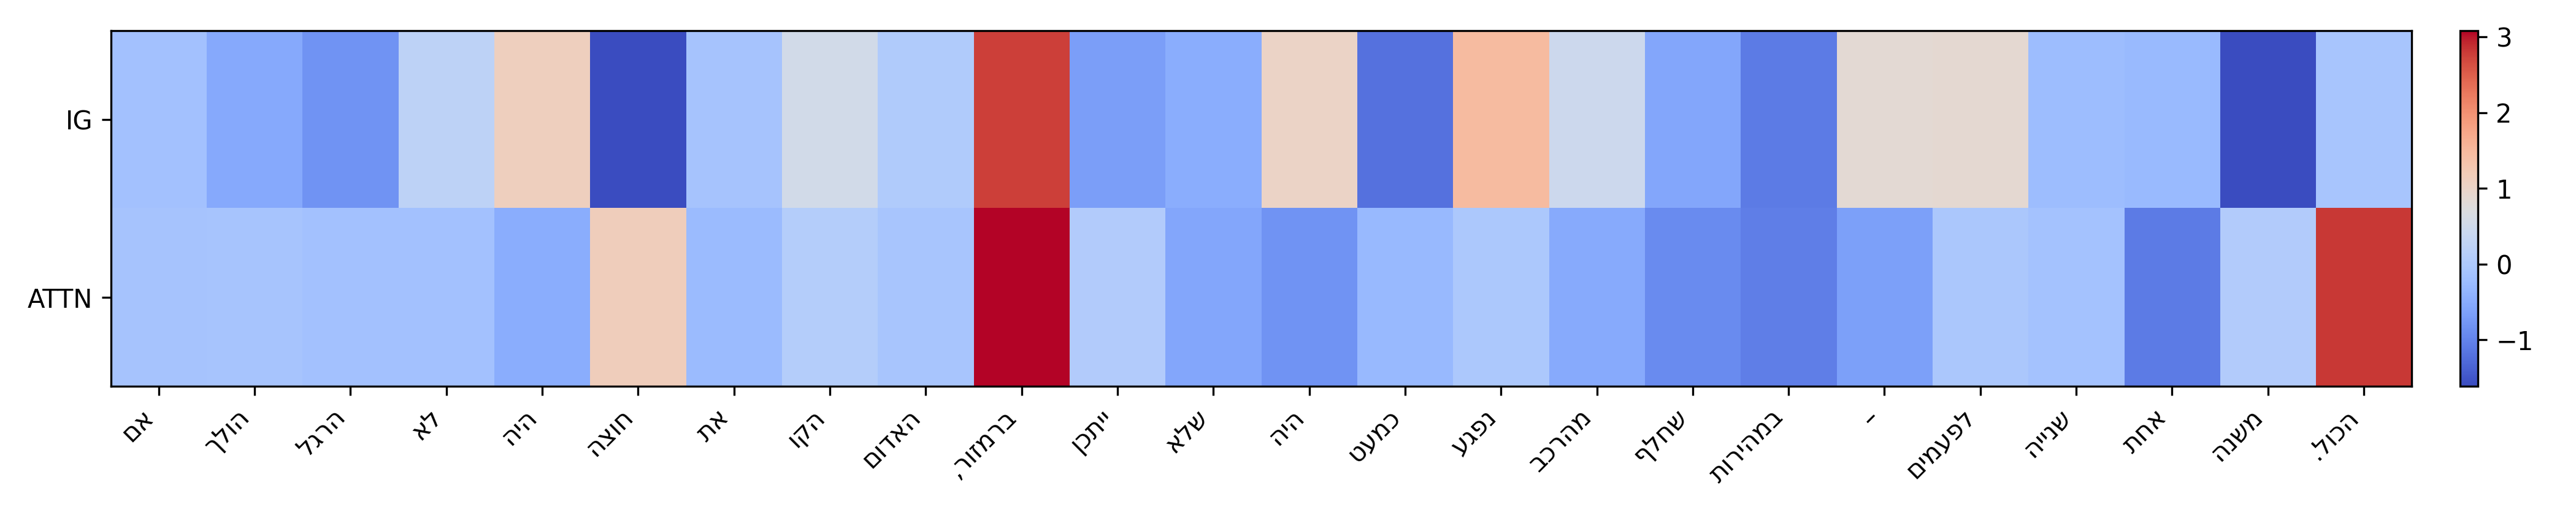
\includegraphics[width=\linewidth]{src/interpretability_partial_end_neodictabert.png}\par\medskip
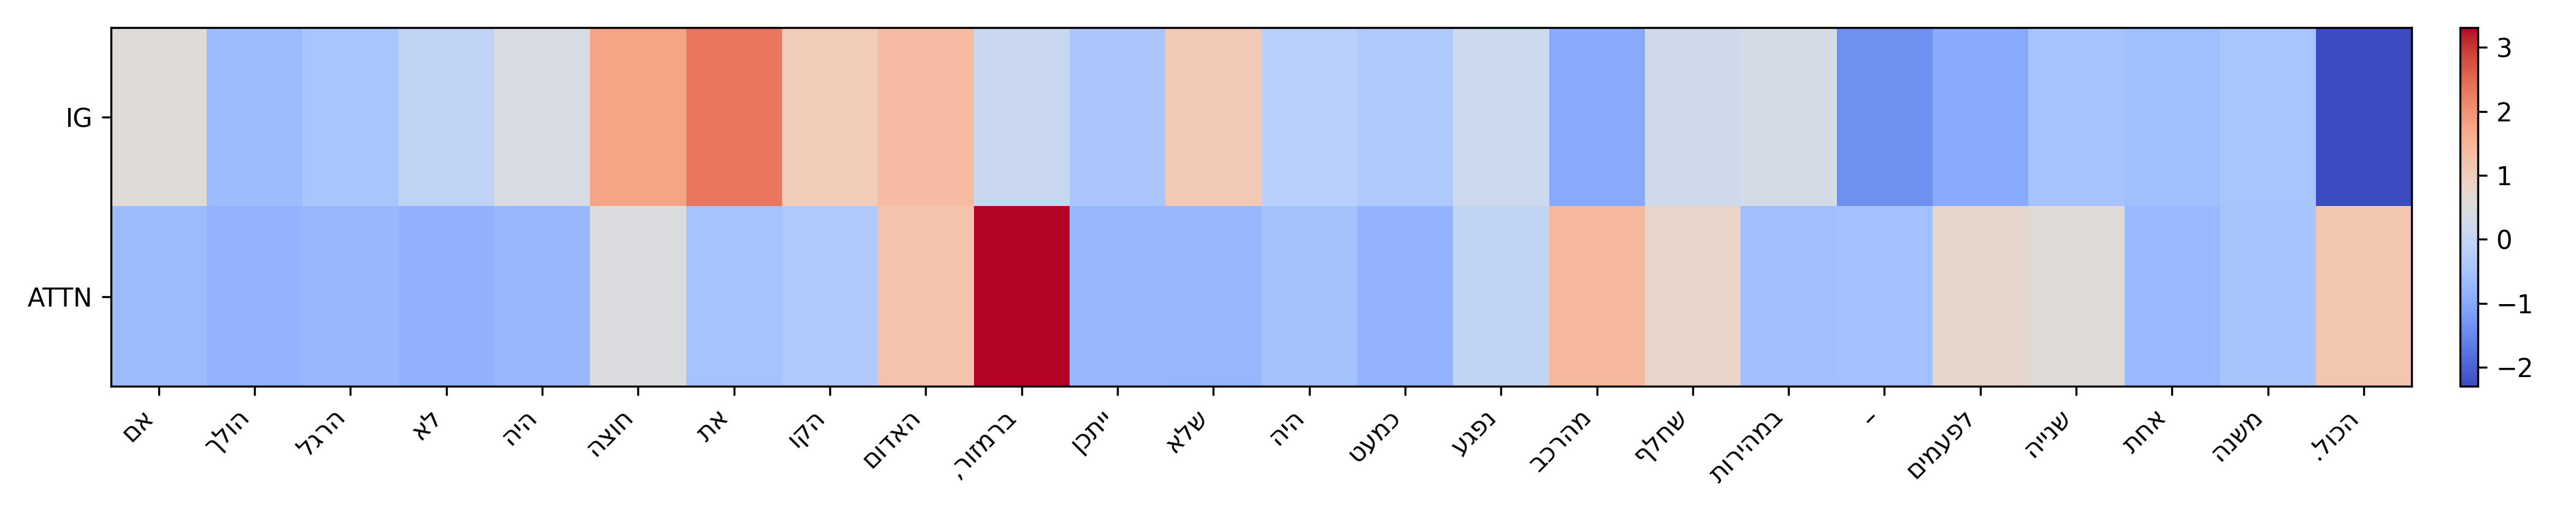
\includegraphics[width=\linewidth]{src/interpretability_partial_end_xlmr.png}
\caption{Representative IG+attention heatmaps for unseen PARTIAL\_END errors: NeoDictaBERT (top) and XLM-RoBERTa (bottom).}
\label{fig:interp_boundary}
\end{figure}

\chapter{Per Idiom SPAN Performance (Unseen)}
\label{sec:appendix_per_idiom}

Table~\ref{tab:per_idiom_unseen} reports mean SPAN F1 for each unseen idiom, averaged across all models and seeds.

\begin{table}[H]
\centering
\small
\renewcommand{\arraystretch}{1.2}
\begin{tabularx}{\linewidth}{@{} L{4cm} X c @{}}
\toprule
\textbf{Unseen Idiom (Hebrew)} & \textbf{Translation} & \textbf{Mean SPAN F1} \\
\midrule
\foreignlanguage{hebrew}{רץ אחרי הזנב של עצמו} & chased own tail & 0.023 \\
\foreignlanguage{hebrew}{נשאר מאחור} & stayed behind & 0.490 \\
\foreignlanguage{hebrew}{חצה קו אדום} & crossed red line & 0.646 \\
\foreignlanguage{hebrew}{שבר שתיקה} & broke silence & 0.919 \\
\foreignlanguage{hebrew}{חתך פינה} & cut corner & 0.945 \\
\foreignlanguage{hebrew}{איבד את הראש} & lost head & 0.991 \\
\bottomrule
\end{tabularx}
\caption{Per idiom SPAN F1 on the unseen test set (mean across models and seeds).}
\label{tab:per_idiom_unseen}
\end{table}

\chapter{Unseen Idiom Selection}
\label{sec:appendix_idioms}

To evaluate zero shot generalization, we held out 6 idioms (480 sentences) entirely from training and validation. These idioms were selected to maximize diversity across four dimensions:

\begin{itemize}
    \item \textbf{Length diversity:} 2--5 tokens, testing span identification across varying idiom lengths
    \item \textbf{Semantic diversity:} Body part, spatial, action, and boundary/threshold metaphors
    \item \textbf{Frequency range:} Common to medium frequency idioms in Hebrew
    \item \textbf{Structural variety:} Different syntactic patterns (verb noun, verb preposition noun, complex clauses)
\end{itemize}

Table~\ref{tab:unseen_idioms} lists each held out idiom with its token count and specific selection rationale.

\begin{table}[H]
\centering
\small
\renewcommand{\arraystretch}{1.2}
\begin{tabularx}{\linewidth}{@{} L{3.2cm} l c X @{}}
\toprule
\textbf{Idiom (Hebrew)} & \textbf{Translation} & \textbf{Tokens} & \textbf{Selection Rationale} \\
\midrule
\foreignlanguage{hebrew}{חתך פינה} & cut corner & 2 & Common idiom with clear literal/figurative distinction; tests basic transfer \\
\foreignlanguage{hebrew}{חצה קו אדום} & crossed red line & 3 & Boundary/threshold metaphor; different semantic category from training idioms \\
\foreignlanguage{hebrew}{נשאר מאחור} & stayed behind & 2 & Spatial metaphor; tests metaphorical spatial reasoning \\
\foreignlanguage{hebrew}{שבר שתיקה} & broke silence & 2 & Very frequent idiom in Hebrew; tests common ``break'' metaphor pattern \\
\foreignlanguage{hebrew}{איבד את הראש} & lost head & 3 & Body part idiom; similar to training idioms but different expression \\
\foreignlanguage{hebrew}{רץ אחרי הזנב של עצמו} & chased own tail & 5 & Longest idiom (5 tokens); tests multi token span identification ability \\
\bottomrule
\end{tabularx}
\caption{The 6 held out idioms for zero shot generalization testing, selected to maximize diversity across length, semantic category, and syntactic structure.}
\label{tab:unseen_idioms}
\end{table}


% --------------------
% Bibliography
% --------------------
\newpage
\bibliographystyle{plainnat}
\label{bib:start}
\bibliography{custom}



% --------------------
% Hebrew Abstract
% --------------------
\clearpage
\begin{otherlanguage}{hebrew}

\chapter*{תקציר}
% No \addcontentsline here — English abstract is already in the TOC.

{\parindent=0pt \parskip=6pt plus 2pt minus 1pt \justifying
\noindent

האם מודלי טרנספורמר \LTR{(Transformer models)} לומדים ייצוגים קומפוזיציוניים של ביטויים אידיומטיים רב מיליים \LTR{(multi word idiomatic expressions)}, או שהם מסתמכים על שינון דפוסים לקסיקליים? עבודה זו בוחנת שאלה זו באמצעות משימת חיזוי גבולות ביטויים אידיומטיים, שבה מודלים נדרשים להכליל ידע מבני לביטויים שלא נראו במהלך האימון.

לשם כך אנו מציגים את מערך הנתונים \LTR{Hebrew Idioms 4800}, מערך נתונים דו משימתי חדש הכולל \LTR{4,800} משפטים המכסים \LTR{60} ביטויים אידיומטיים, עם הסכמה בין מתייגים כמעט מושלמת \LTR{(Cohen’s $\kappa = 0.97$)}. אנו מעריכים שישה מקודדי טרנספורמר \LTR{(Transformer encoders)} וחמישה מודלי שפה גדולים \LTR{(large language models)} בשתי משימות משלימות: סיווג שימוש בביטויים אידיומטיים \LTR{(classification, CLS)} וזיהוי ביטויים אידיומטיים ברמת הטוקן \LTR{(span identification, SPAN)} באמצעות תיוג \LTR{(BIO tagging)}, הן עבור ביטויים אידיומטיים שנראו באימון והן עבור ביטויים אידיומטיים שלא נראו באימון.

תוצאות הניסוי מצביעות על פער משמעותי בין המשימות. בעוד שסיווג שימוש בביטויים אידיומטיים מכליל היטב לביטויים אידיומטיים שלא נראו באימון, עם \LTR{F1 0.90--0.92} וירידה של \LTR{0.5--3.5} נקודות בלבד, ביצועי זיהוי הגבולות נפגעים באופן ניכר עם \LTR{F1 0.59--0.76} וירידה של \LTR{23--41} נקודות. ניתוח השגיאות חושף כשלים שיטתיים בזיהוי גבולות ביטוי אידיומטי: קיצוצי סוף ביטוי \LTR{(partial end truncations)} הם מקור הטעות המרכזי במודלים שעברו אימון עדין \LTR{(fine tuning)}, ובביטויים אידיומטיים ארוכים שלא נראו באימון \LTR{(5+ tokens)} שיעורי השגיאה מגיעים ל־\LTR{70--100\%}, למרות ביצועים כמעט מושלמים על ביטויים אידיומטיים מוכרים.

לעומת זאת, שימוש בפרומפטים \LTR{(prompting)} במודלי שפה גדולים מציג דפוס שגיאות שונה ויכולת הכללה עדיפה. קיצוצי תחילה \LTR{(partial start truncations)} מופיעים בתדירות גבוהה יותר בגישת הפרומפטים, ומודל \LTR{Gemini 3 Flash} מגיע ל־\LTR{SPAN F1 90\%} על ביטויים אידיומטיים שלא נראו באימון, תוצאה הגבוהה מביצועי המודל המאומן הטוב ביותר \LTR{76.1\%}. ממצאים אלה מצביעים על כך שאימון עדין עשוי לעודד שינון גבולות ביטוי אידיומטי, בעוד שימוש בפרומפטים שומר במידה רבה יותר על הסקה קומפוזיציונית.

ממצאים אלו מלמדים כי מודלי טרנספורמר שעברו אימון עדין מסוגלים לסווג אידיומטיות על בסיס דפוסי פני שטח, אך מתקשים ללמוד רמזים קומפוזיציוניים לזיהוי גבולות ביטויים אידיומטיים, וכי שימוש בפרומפטים עשוי להוות חלופה יעילה יותר להכללה לביטויים אידיומטיים חדשים.


\vspace{1cm}
}
\end{otherlanguage}
\clearpage



% --------------------
% Hebrew Supervision Note
% --------------------
\clearpage
\thispagestyle{empty}
\vspace*{\fill}
\begin{center}
\begin{otherlanguage}{hebrew}
עבודה זו בוצעה תחת הנחייתו של ד"ר כפיר בר\\
מבית הספר למדעי המחשב ע"ש אפי ארזי, אוניברסיטת רייכמן
\end{otherlanguage}
\end{center}
\vspace*{\fill}
\clearpage



% --------------------
% Hebrew Title Page
% --------------------
\hypersetup{pageanchor=false}   % avoid duplicate page.1 anchor (English title page already created one)
\begin{titlepage}
\centering
\vspace*{2cm}

\begin{otherlanguage}{hebrew}

% --- University + Program (Hebrew) ---
{\Large אוניברסיטת רייכמן\par}
\vspace{0.3cm}
{\large בית ספר אפי ארזי למדעי המחשב\par}
{\large מסלול \LTR{MLDS} \LTR{(M.Sc.)}\, - התוכנית לתואר שני\par}

\vspace{3cm}

% --- Title (Hebrew) ---
{\LARGE \bfseries זיהוי ללא לוקליזציה: כשלי הכללה קומפוזיציונית במודלי טרנספורמר בגבולות ביטויים אידיומטיים בעברית\par}
\vspace{0.5cm}
{\large בניית מערך נתונים והערכת מודלים באמצעות אימון עדין ופרומפטינג\par}

\vspace{3cm}

% --- Author (Hebrew) ---
{\large מאת\par}
{\Large איגור נזרנקו ויובל עמית\par}

\vspace{3cm}

% --- Submission Note (Hebrew) ---
{\normalsize
  עבודה זו מוגשת כחלק מהדרישות לשם קבלת תואר מוסמך~\LTR{M.Sc.}\  במסלול
 \LTR{MLDS} בבית ספר אפי ארזי למדעי המחשב, אוניברסיטת רייכמן
\par}

\vspace{2cm}

% --- Date (Hebrew) ---
{\Large פברואר \LTR{2026}\par}

\end{otherlanguage}

\end{titlepage}


\end{document}
